\documentclass[a4paper]{article}
\usepackage{graphicx}
\usepackage{twocolceurws}


\title{Specified Backup for Fragile Parts of LLMs}

\author{
Abhi Morumpalle
\and
Allen Zhang
\and
Arnav Marda
\and
Jeffrey Kwan
\and
Harry Qian
}

\institution{Team A5}




\begin{document}
\maketitle

\begin{abstract}
In the past few years, there has been an explosion of interest in Large Language Models (LLMs) for a variety of practical applications. Much of this explosion has been driven by the invention of the Transformer architecture. However, the Transformer architecture inner workings largely remain a mystery. Combining this with the applications that LLMs are finding in the real-world, there a variety of new security risks that these LLMs open
up their users to. In this paper, we analyze the robustness of LLMs to random bitflips in the variables, pinpointing specific parts of the LLM that are vulnerable to these hardware errors.


\end{abstract}


\section{Introduction}

In the past few years, there has been an explosion of interest in LLMs with the creation of widely available resources like OpenAI's ChatGPT
and Meta's open source Llama. Much of the explosion has been driven by the creation of the transformer architecture, which has made a dramatic difference throughout AI, but particularly in the world of LLMs. However, our fundamental understanding of how these objects remains shrouded in mystery.

Because of our lack of understanding of how these objects work, and the quick assimilation of these products into our daily lives, there are a variety of novel security risks that we are being introduced to. One specific error is not so common, but still of practical relevance, is a hardware failure in which a random bitflip occurs in the parameters of our model. An error of such a fashion could have drastic effects on our output, ranging from making the outputs gibberish to outright wrong.

In this paper, we analyze how injecting bit errors into specific locations of a transformer and the LLM model as a whole affect the output. To this end, we use the \{INSERT MODEL\} as a base model to test on. To inject errors into our base model we use the PyTEI package \cite{Ma23}. To quantify the effect of our errors, we compare the score of our base model to the score of the models with errors injected using the \{INSERT TESTS\}.

Our basic workflow is outlined in the below diagram

\begin{figure}[ht]
	\begin{center}
		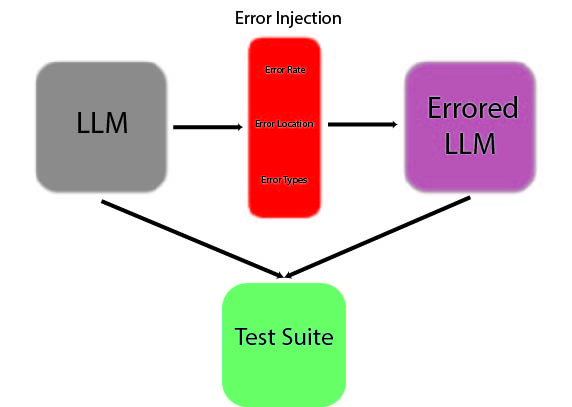
\includegraphics[height=6cm]{workflow.jpg}
		\caption{General evaluation workflow for LLM}
		\label{workflow}
	\end{center}
\end{figure}
\section{Project Goals and Timeline}

The goal of this project is to evaluate the effect of random bit flips on the output of LLMs and analyze the possible security hazards that these hardware errors could cause in real systems. We plan to do this by modeling various rates of bit flips and by injecting errors into various parts of the LLMs, and evaluating the robustness on a variety of different tests.

Up until now, we have chosen a open source model that gives us the freedom to inject various bit errors, and have select some tests that we can evaluate our models on. There are still multiple tests that we want to evaluate our model on, and some more analysis to be done to find specific places to inject bit flips into to look for any particularly vulnerable parts.

Below is a general timeline for what we want to accomplish and when.

\begin{itemize}
	\item Week 7: Finish selecting different tests to evaluate
	\item Week 8: Try injecting vulnerabilities into specific parts of the LLM with different error rates
	\item Week 9: Analyze results and compile into final report
	\item  Week 10: Finish final report and presentation
\end{itemize}

Using this, we can turn the knobs to evaluate different kinds of error and add various tests to our test-suite as we continue to expand our results.

\section{Methods}
We chose Hugging Face's implementations of GPT-2 as our model of choice. We evaluated our models on DeepEval, an open-source LLM benchmark, specifically the computer science and astronomy tests that have the injected LLM answer multiple choice questions. For each model with varying error rates, the score is computed as the proportions of correct answers. For the purposes of this midterm report, we only implemented coarsed-grained error injection into every layer.


[TODO: citations for the models and the benchmark]

\section{Preliminary Results}
\begin{figure}[ht]
	\begin{center}
		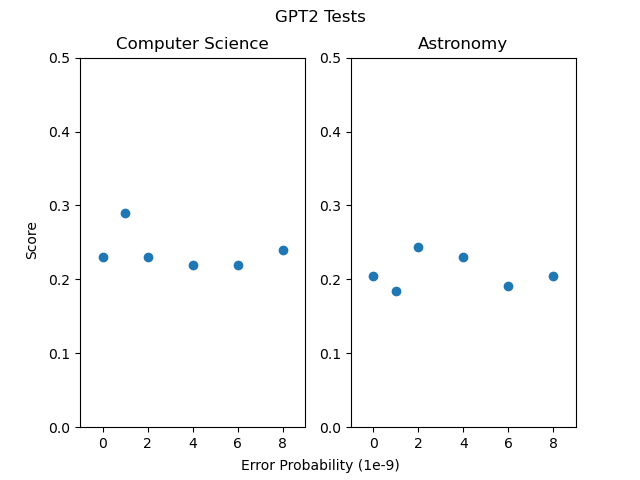
\includegraphics[height=6cm]{gpt2.png}
		\caption{GPT 2 performance on DeepEval with varying error rates}
		\label{gpt2-res}
	\end{center}
\end{figure}

As seen in Figure \ref{gpt2-res}, we see a negligable change in performance varying error rates in the range of 1e-9 on both benchmarks. Note that we were unable to increase the error rate anything beyond that because it resulted in a NaN output. This is likely due to the fact that random bit flips happened in the exponent field of a number.

\section{Future Work}

In the near future, we hope to be able to pick more tests that can evaluate the effect of bit flips on our model. This will take a significant amount of compute time, even though we have chosen a mini LLM model.

For future work, we hope to be able to analyze our different parts of the LLM are affected by random bit flips. For example, we want to see if a bit flip in the attention mechanism is more relevant than a bit flip in the fully connected layeres, or vice versa. 

In addition, because of the bits being stored as a floating point, it's also possible that some bit flips can be much more relevant than others. For example, a bit being flipped in the exponent produces a much larger effect than a bit being flipped in the mantissa. We hope to be able to expand on the PyTEI library to give us the ability to evaluate these effects.

Using this larger body of results, we hope to be able to analyze the possible security risks that hardware errors pose to LLM implementations.

\section{Related Work}
There is a related paper \cite{Ma23} that analyzes a model known as a recommendation system. In their work, they build the PyTEI package for injecting models. However, recommendation models differ significantly from LLMs so the overall effect could be quite different for the same error injections.

However, the paper does not do any evaluation on the different of hardware errors in specific parts of the recommendation system, so the question of whether particular parts are more vulnerable is still open.

An interesting part of this paper is the evaluation of possible mitigations against hardware flips, which can also be evaluated in the context of LLMs. In addition, their evaluation had limited scope, and it could be interesting to expand on their analysis by testing a wider variety of errors and examining the tradeoffs of each.

\section{First Level Heading}

First level headings are all flush left, initial caps, bold and in point
size 12. One line space before the first level heading and $1/2$ line
space after the first level heading.

\subsection{Second Level Heading}

Second level headings must be flush left, initial caps, bold and in point
size 10. One line space before the second level heading and $1/2$ line
space after the second level heading.

\subsubsection{Third Level Heading}

Third level headings must be flush left, initial caps and bold.
One line space before the third level heading and $1/2$ line
space after the third level heading.

\paragraph{Fourth Level Heading}

Fourth level headings must be flush left, initial caps and roman type.
One line space before the fourth level heading and $1/2$ line
space after the fourth level heading.

\subsection{Citations In Text}

Citations within the text should indicate the author's last name and
year\cite{Knuth-vol3}. Reference style\cite{Comer-btree}
should follow the style that you are used to using, as long as the
citation style is consistent.

\subsubsection{Footnotes}

Indicate footnotes with a number in
the text. Place the footnotes at the bottom of the page they appear on.
Precede the footnote with a vertical rule of 2 inches (12 picas).

\subsubsection{Figures}

All artwork must be centered, neat, clean and legible. Do not use pencil
or hand-drawn artwork. Figure number and caption always appear after the
the figure. Place one line space before the figure, one line space
before the figure caption and one line space after the figure caption.
The figure caption is initial caps and each figure is numbered
consecutively.

Make sure that the figure caption does not get separated from the
figure. Leave extra white space at the bottom of the page to avoid
splitting the figure and figure caption.

Figure \ref{fig1} shows how to include a figure as encapsulated postscript.
The source of the figure is in file {\tt fig1.eps}.

\begin{figure}[ht]
\begin{center}
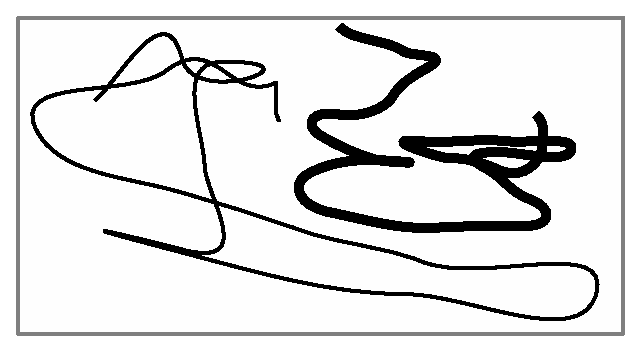
\includegraphics[height=4cm]{fig1}
\caption{Sample EPS figure }
\label{fig1}
\end{center}
\end{figure}

Below is another figure using LaTeX commands.


\begin{figure}[ht]
\begin{center}
\setlength{\unitlength}{1pt}
\footnotesize
\begin{picture}(160,80)
        \put(0,0){\framebox(160,80)[]{}}
        \put(10,35){\framebox(80,40){}}
        \put(100,20){\framebox(40,20){}}
        \put(70,10){\framebox(20,10){}}
        \put(20,5){\framebox(10,5){}}
\end{picture}
\caption{Sample Figure Caption}
\end{center}
\end{figure}

\subsubsection{Tables}

All tables must be centered, neat, clean and legible. Do not use pencil
or hand-drawn tables. Table number and title always appear before the
table.

One line space before the table title, one line space after the table
title and one line space after the table. The table title must be
initial caps and each table numbered consecutively.

\begin{table}[ht]
\begin{center}
\caption{Sample Table}

\bigskip

\begin{tabular}{|l|l|r|}
\hline
A & B & 1\\ \hline
C & D & 2\\
E & F & 3\\ \hline
\end{tabular}
\end{center}
\end{table}


\subsubsection{Handling References}

Use a first level heading for the references. References follow the
acknowledgements.


\subsubsection{Acknowledgements}

Use a third level heading for the acknowledgements. All acknowledgements
go at the end of the paper.




%\bibliographystyle{alpha} 
%\bibliography{samplebib}
%inline the .bbl file directly for mailing to authors.

\begin{thebibliography}{Com79}
\bibitem[Ma et al., 2023]{Ma23} D. Ma, X. Jiao, F. Lin, M. Zhang, A. Desmaison, T. Sellinger, D. Moore, S. Sankar.
\newblock Evaluating and Enhancing Robustness of Deep Recommendation Systems Against Hardware Errors

\end{thebibliography}

\end{document}


